% !TeX document-id = {f19fb972-db1f-447e-9d78-531139c30778}
% !BIB program = biber
\documentclass{beamer}
%\documentclass[handout]{beamer}

%\usetheme{focus}
%\usepackage[style=authoryear]{biblatex}
%\renewcommand*{\nameyeardelim}{\addcomma\addspace}
\usepackage[T1]{fontenc}
\usetheme[block=fill,subsectionpage=progressbar,sectionpage=none]{metropolis} 
%\usepackage[natbibapa]{apacite}
\usepackage{wasysym}
\usepackage{etoolbox}
\usepackage[utf8]{inputenc}

\usepackage{threeparttable}
\usepackage{subcaption}

\usepackage{tikz-qtree}
\setbeamercovered{still covered={\opaqueness<1->{5}},again covered={\opaqueness<1->{100}}}

 
\usepackage[american]{babel}
\usepackage{csquotes}
\usepackage[style=apa, backend = biber]{biblatex}
\DeclareLanguageMapping{american}{american-UoN}
\addbibresource{../../bdaca.bib}
\renewcommand*{\bibfont}{\tiny}

\usepackage{tikz}
\usetikzlibrary{shapes,arrows,matrix}
\usepackage{multicol}

 
\makeatletter
\setbeamertemplate{headline}{%
  \begin{beamercolorbox}[colsep=1.5pt]{upper separation line head}
  \end{beamercolorbox}
  \begin{beamercolorbox}{section in head/foot}
    \vskip2pt\insertnavigation{\paperwidth}\vskip2pt
  \end{beamercolorbox}%
  \begin{beamercolorbox}[colsep=1.5pt]{lower separation line head}
  \end{beamercolorbox}
}
\makeatother

 

\setbeamercolor{section in head/foot}{fg=normal text.bg, bg=structure.fg}



\newcommand{\question}[1]{
	\begin{frame}[plain]
		\begin{columns}
			\column{.3\textwidth}
			\makebox[\columnwidth]{
				\includegraphics[width=\columnwidth,height=\paperheight,keepaspectratio]{../../pictures/mannetje.png}}
			\column{.7\textwidth}
			\large
			\textcolor{orange}{\textbf{\emph{#1}}}
		\end{columns}
\end{frame}}




\title[Big Data and Automated Content Analysis]{\textbf{Big Data \& Automated Content Analysis} \\ Week 1 -- Wednesday: »Introduction«}
\author[Damian Trilling]{Damian Trilling \\ ~ \\ \footnotesize{d.c.trilling@uva.nl \\@damian0604} \\ \url{www.damiantrilling.net}}
\date{3 February 2021}
\institute[UvA]{Afdeling Communicatiewetenschap \\Universiteit van Amsterdam}

\begin{document}

\begin{frame}{}
\titlepage
\end{frame}

\begin{frame}{Today}
\tableofcontents
\end{frame}


\section{Getting to know each other}

\begin{frame}{Damian}

	\begin{columns}
		\column{.3\textwidth}
		\makebox[\columnwidth]{
			\includegraphics[width=\columnwidth,height=\paperheight,keepaspectratio]{../../pictures/damian.jpg}}
		\column{.7\textwidth}
		dr. Damian Trilling \\
        Universitair Hoofddocent (Associate Professor) Communication in the Digital Society \\
		\begin{itemize}
			\item studied Communication Science in M\"unster and at the VU 2003--2009
			\item PhD candidate @ ASCoR 2009--2012
			\item political communication and journalism in a changing media environment
			\item computational research methods
		\end{itemize}
		@damian0604 ~~ d.c.trilling@uva.nl ~~ REC-C~8\textsuperscript{th}~floor ~~ \url{www.damiantrilling.net} 
	\end{columns}
\end{frame}


\begin{frame}{Vlad}
	\begin{columns}
		\column{.3\textwidth}
		\makebox[\columnwidth]{
			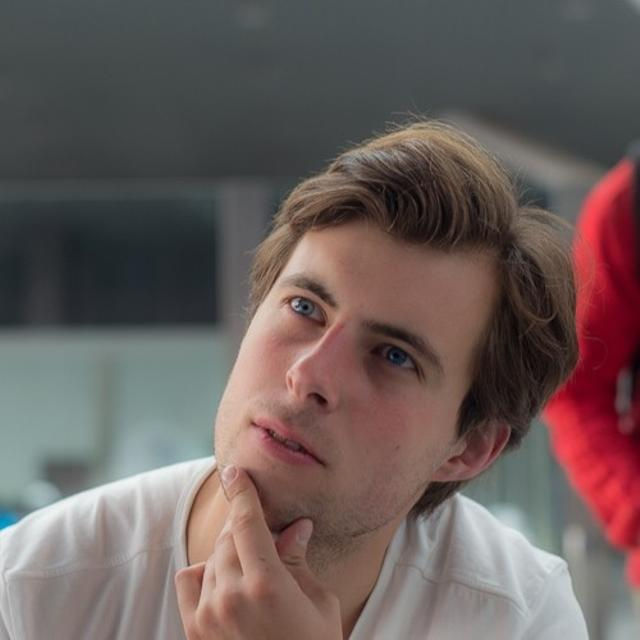
\includegraphics[width=\columnwidth,height=\paperheight,keepaspectratio]{../../pictures/vlad.jpg}}
		\column{.7\textwidth}
		Vladislav Petkevic \\
		Junior Lecturer Communication Science \\
		\begin{itemize}
			\item MSc in Communication Research (2020)
			\item Interested in politicial communication, especially election campaigns
			\item Even more interested in applying computational research methods (e.g. NLP, maschine vision) to studying social phenomena
		\end{itemize}
		v.petkevich@uva.nl
	\end{columns}
\end{frame}




\begin{frame}{You}
	\begin{columns}
		\column{.3\textwidth}
		\makebox[\columnwidth]{
			\includegraphics[width=\columnwidth,height=\paperheight,keepaspectratio]{../../pictures/mannetje.png}}
		\column{.7\textwidth}
		Your name?\\
		Your background?\\
		Your reason to follow this course?
	\end{columns}
\end{frame}



\section{Setting the stage}

\subsection{Defining ``Big Data''}

{\setbeamercolor{background canvas}{bg=black}
	\begin{frame}[plain]
		\makebox[\linewidth]{
			\includegraphics[width=\paperwidth,height=\paperheight,keepaspectratio]{../../pictures/bigdataisliketeenagesex.jpg}
		}
	\end{frame}
}

\begin{frame}{The ``pragmatic'' definition }
	\begin{block}{}
Everything that needs so much computational power and/or storage that you cannot do it on a regular computer.
	\end{block}
\end{frame}



\begin{frame}{The ``commercial'' definition }
	\begin{block}{\textcite{gartner}}
``Big data is high-volume, high-velocity and/or high-variety information assets that demand cost-effective, innovative forms of information processing that enable enhanced insight, decision making, and process automation.''
	\end{block}
\end{frame}



\begin{frame}{The ``critical'' definition }
	\begin{block}{\textcite{boyd2012}}
``
	\begin{enumerate}
		\item Technology: maximizing computation power and algorithmic accuracy to gather, analyze, link, and compare large data sets.
		\item Analysis: drawing on large data sets to identify patterns in order to make economic, social, technical, and legal claims.
		\item Mythology: the widespread belief that large data sets offer a higher form of intelligence and knowledge that can generate insights that were previously impossible, with the aura of truth, objectivity, and accuracy.
	\end{enumerate}
''
	\end{block}
\end{frame}




\question{Do you think we are doing Big Data analysis?}




\subsection{Defining Computational (Social|Communication) Science}



\begin{frame}{A very young field}
	\begin{block}{\textcite{Lazer2009}}
		``The capacity to collect and analyze massive amounts of data has transformed such fields as biology and physics. But the emergence of a data-driven `computational social science' has been much slower.''
	\end{block}
\end{frame}




\begin{frame}{Epistemologies and paradigm shifts}
	\begin{block}{\textcite{Kitchin2014}}<1->
		\begin{itemize}
			\item<2-> (Reborn) empiricism: purely inductive, correlation is enough
			\item<3-> Data-driven science: knowledge discovery guided by theory
			\item<4-> Computational social science and digital humanities: employ Big Data research within existing epistemologies
			\begin{itemize}
				\item DH: descriptive statistics, visualizations
				\item CSS: prediction and simulation
			\end{itemize}
		\end{itemize}
	\end{block}
\end{frame}




\begin{frame}{CCS as a subset of CSS}
	\begin{block}{\textcite{Hilbert2019}}
		``\ldots our definition of computational communication science as an application of computational science to questions of human and social communication. As such, it is a natural subfield of computational social science'' (followed by references to CSS definitions)
	\end{block}
\end{frame}



\begin{frame}{Data, analysis, theory}
	\begin{block}{\textcite{VanAtteveldt2018a}}
		``\ldots computational communication science studies generally involve: (1) large and complex data sets; (2) consisting of digital traces and other ``naturally occurring'' data; (3) requiring algorithmic solutions to analyze; and (4) allowing the study of human communication by applying and testing communication theory.''
	\end{block}	
	
\end{frame}



\question{
	\begin{enumerate}
		\item 	What do you think? What is the essence of Big Data/CSS/CCS?
		\item How will what we do here relate to theories and methods from other courses?
	\end{enumerate}
}





\section{The toolbox}
\subsection{The role of software in CSS}



\begin{frame}{Why program your own tool?}
\begin{block}{\textcite{Vis2013}}
	``Moreover, the tools we use can limit the range of questions that might be imagined, simply because they do not fit the affordances of the tool. Not many researchers themselves have the ability or access to other researchers who can build the required tools in line with any preferred enquiry. This then introduces serious limitations in terms of the scope of research that can be done.''	
\end{block}

\end{frame}


\begin{frame}{Some considerations regarding the use of software in science}
	Assuming that science should be \emph{transparent} and \emph{reproducible by anyone}\onslide<2->{, we should}
	\begin{block}{use tools that are}<2->
		\begin{itemize}
			\item platform-independent 
			\item free (as in beer and as in speech, gratis and libre)
			\item which implies: open source
		\end{itemize}
	\end{block}
	\onslide<3>{This ensures it can our research (a) can be reproduced by anyone, and that there is (b) no black box that no one can look inside. $\Rightarrow$ ongoing open-science debate! \parencite{VanAtteveldt2019}}
\end{frame}

\begin{frame}{Why program your own tool?}
\begin{block}{\textcite{Vis2013}}
``{[}\ldots{]} these {[}commercial{]} tools are often unsuitable for academic purposes because of their cost, along with the problematic `black box' nature of many of these tools.''
\end{block}

\begin{block}{\textcite{Mahrt2013}}
``{[}\ldots{]} we should resist the temptation to let the opportunities and constraints of an application or platform determine the research question {[}\ldots{]}''
\end{block}
	
\end{frame}






\subsection{Python: A language, not a program}


\begin{frame}[plain]
	\makebox[\columnwidth]{
		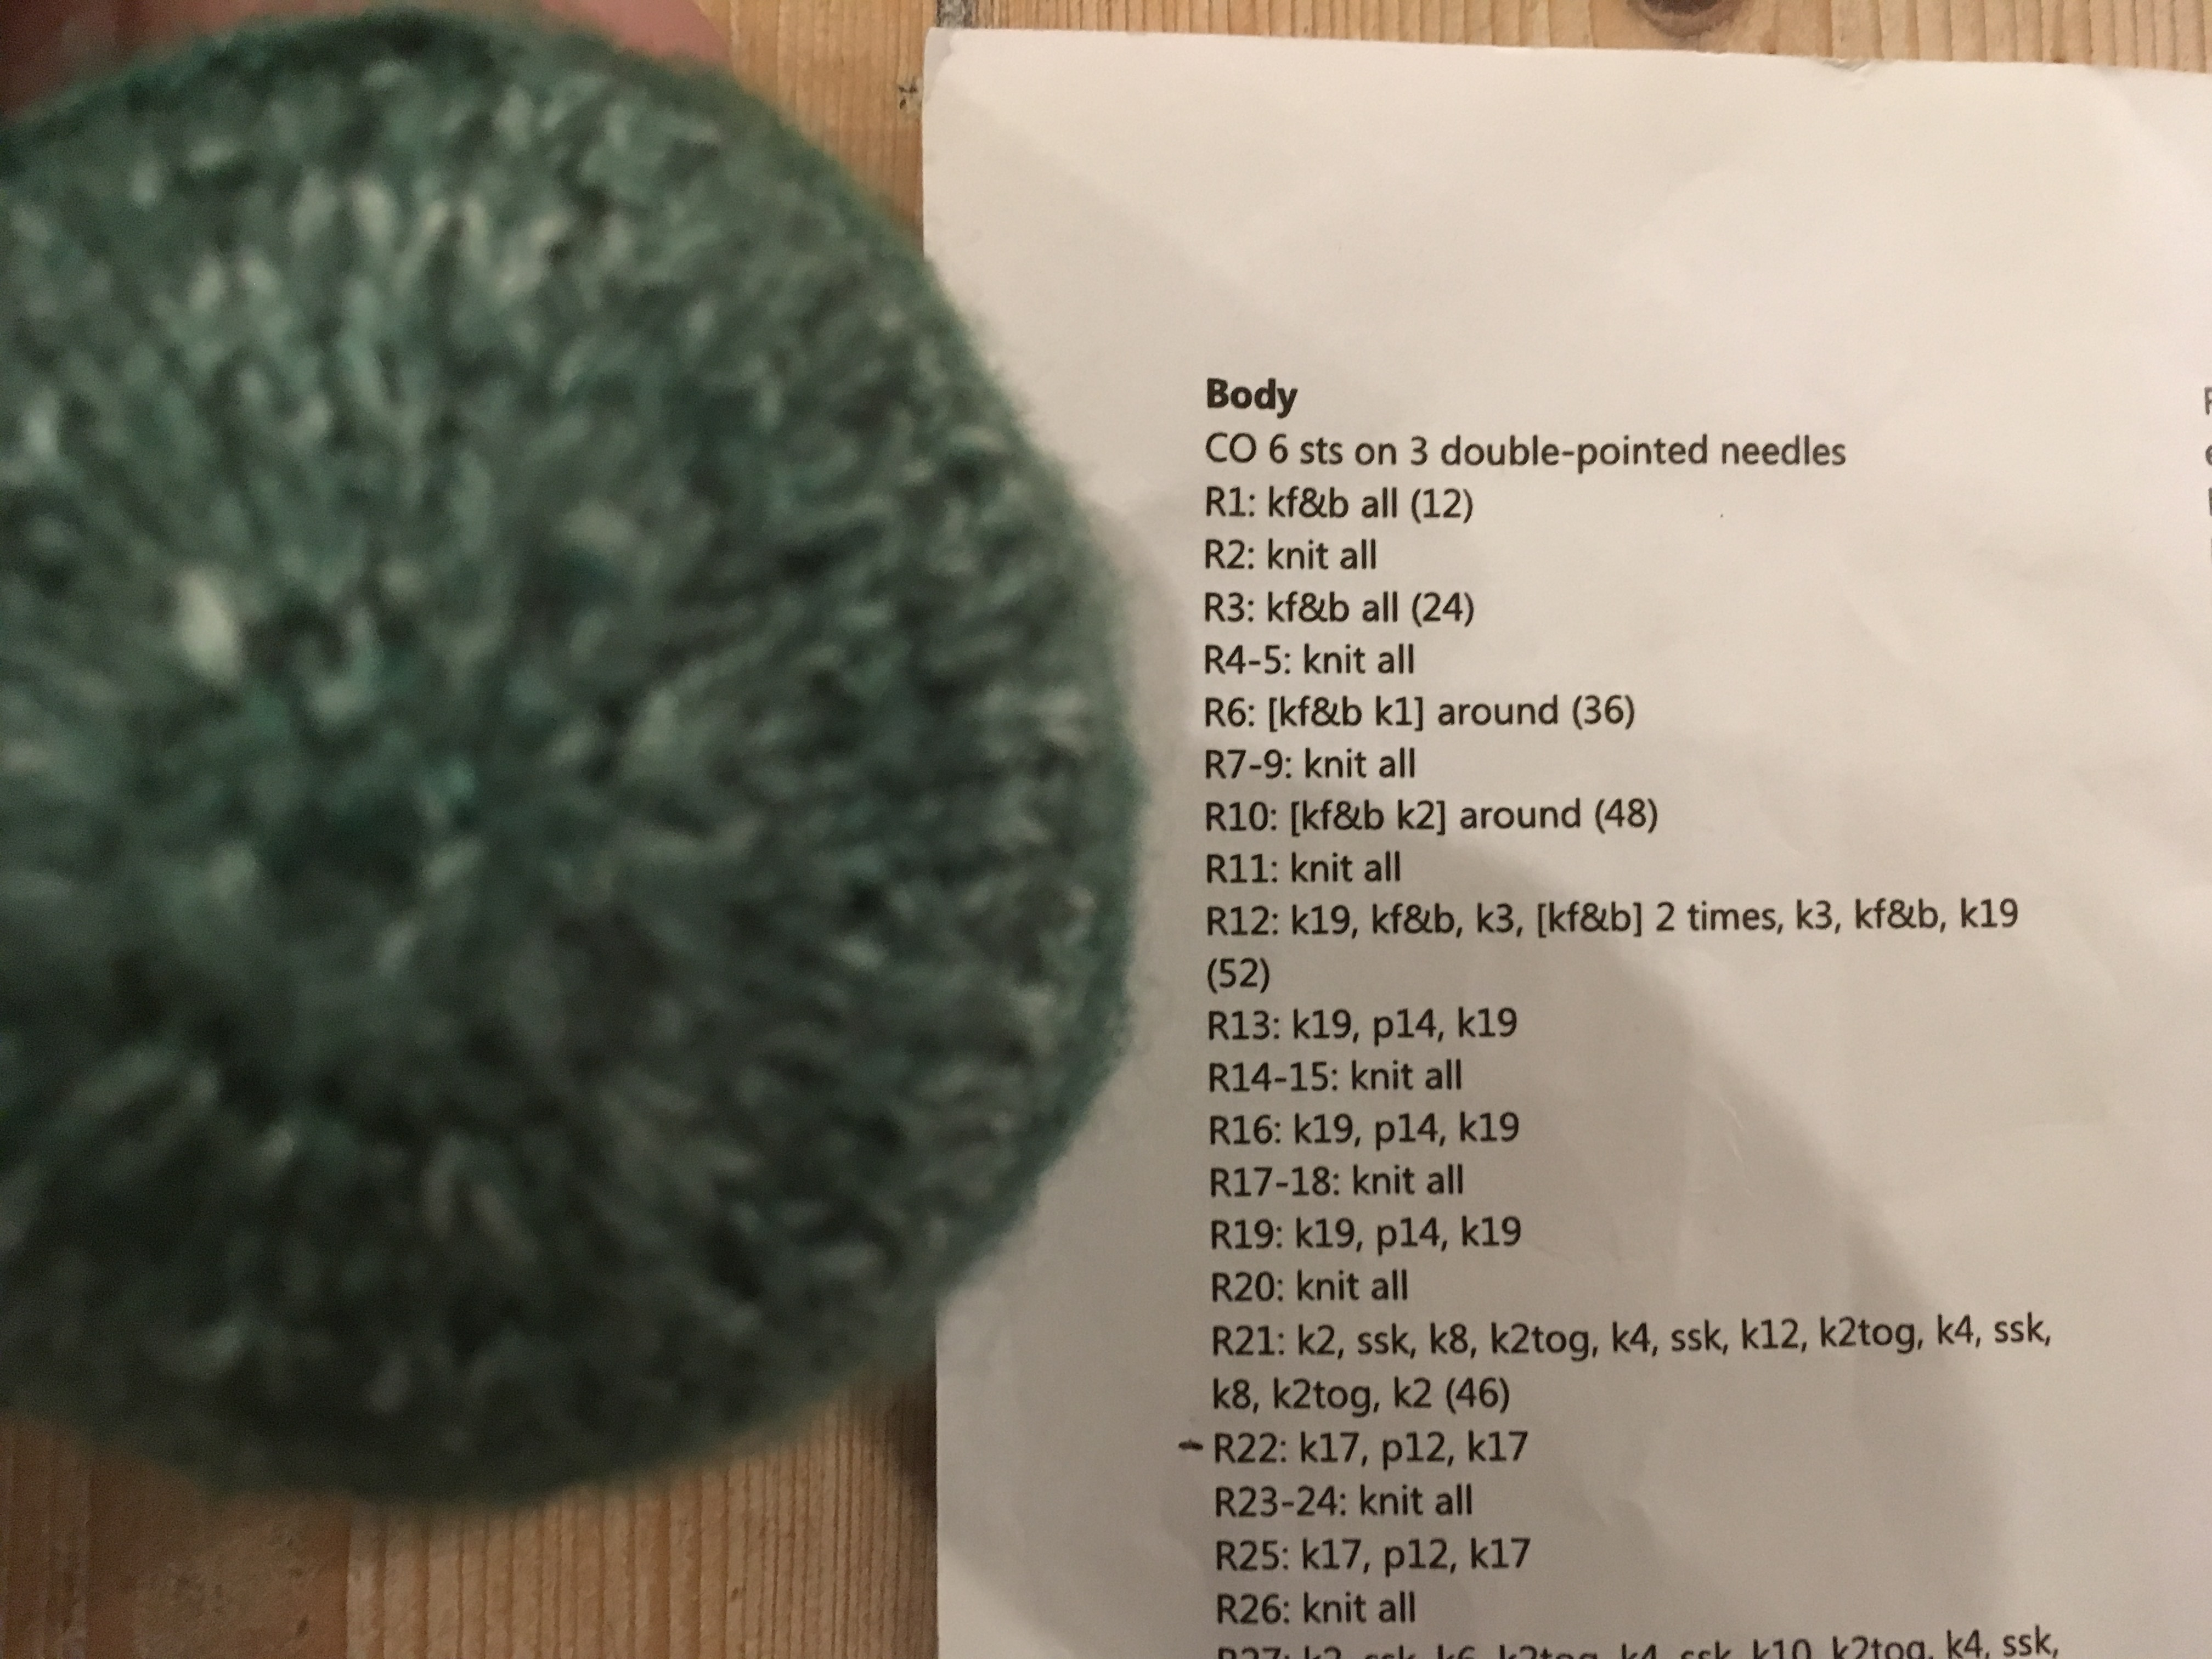
\includegraphics[width=\columnwidth,height=\paperheight,keepaspectratio]{../../pictures/knitting.jpg}}
	\footnotesize{An algorithm in a language that's a bit harder (I think) than Python}
\end{frame}



\begin{frame}{Python}
	\begin{block}{What?}<1->
		\begin{itemize}
			\item A language, not a specific program
			\item Huge advantage: flexibility, portability
			\item One of \emph{the} languages for data analysis. \tiny{(The other one is R.)}
			\onslide<2>{ \\\tiny{But Python is more flexible---the original version of Dropbox was written in Python. Some people say: R for numbers, Python for text and messy stuff.}}
		\end{itemize}
	\end{block}
	
	\begin{block}{Which version?}<3->
		We use Python 3. \\ 
		\footnotesize{\url{http://www.google.com} or \url{http://www.stackexchange.com} still may show you some Python2-code, but that can easily be adapted. Most notable difference: In Python 2, you write {\tt print "Hi"}, this has changed to {\tt print ("Hi")}.}\\
	\end{block}
\end{frame}

\begin{frame}[standout]
	Make sure you can run Python code and install packages. Otherwise, you won't be able to follow along on Friday. (See instructions you got. Use Vlad's office hours if you cannot figure it out.))
\end{frame}


\begin{frame}[plain]
    \printbibliography
\end{frame}

\end{document}
